% Metódy inžinierskej práce

\documentclass[10pt,twoside,english,a4paper]{article}

\usepackage[english]{babel}
%\usepackage[T1]{fontenc}
\usepackage[IL2]{fontenc} % lepšia sadzba písmena Ľ než v T1
\usepackage[utf8]{inputenc}
\usepackage{graphicx}
\usepackage{url} % príkaz \url na formátovanie URL
\usepackage{hyperref} % odkazy v texte budú aktívne (pri niektorých triedach dokumentov spôsobuje posun textu)

\usepackage{cite}
%\usepackage{times}

\pagestyle{headings}

\title{Recommendation systems for personalized advertising in digital marketing\thanks{Semestral project in the subject Methods of engineering work, academic year 2024/25, supervised by Pavol Batalik}} % meno a priezvisko vyučujúceho na cvičeniach

\author{Vsevolod Salik\\[2pt]
	{\small Slovak University of Technology in Bratislava }\\
	{\small Faculty of Informatics and Information Technologies }\\
	{\small \texttt{xsalik@stuba.sk}}
	}

\date{\small 26. september 2024} % upravte



\begin{document}

\maketitle

\begin{abstract}
\ldots
\end{abstract}



\section{Introduction}
Test

%\begin{figure}[h!]
%\begin{subfigure}
  %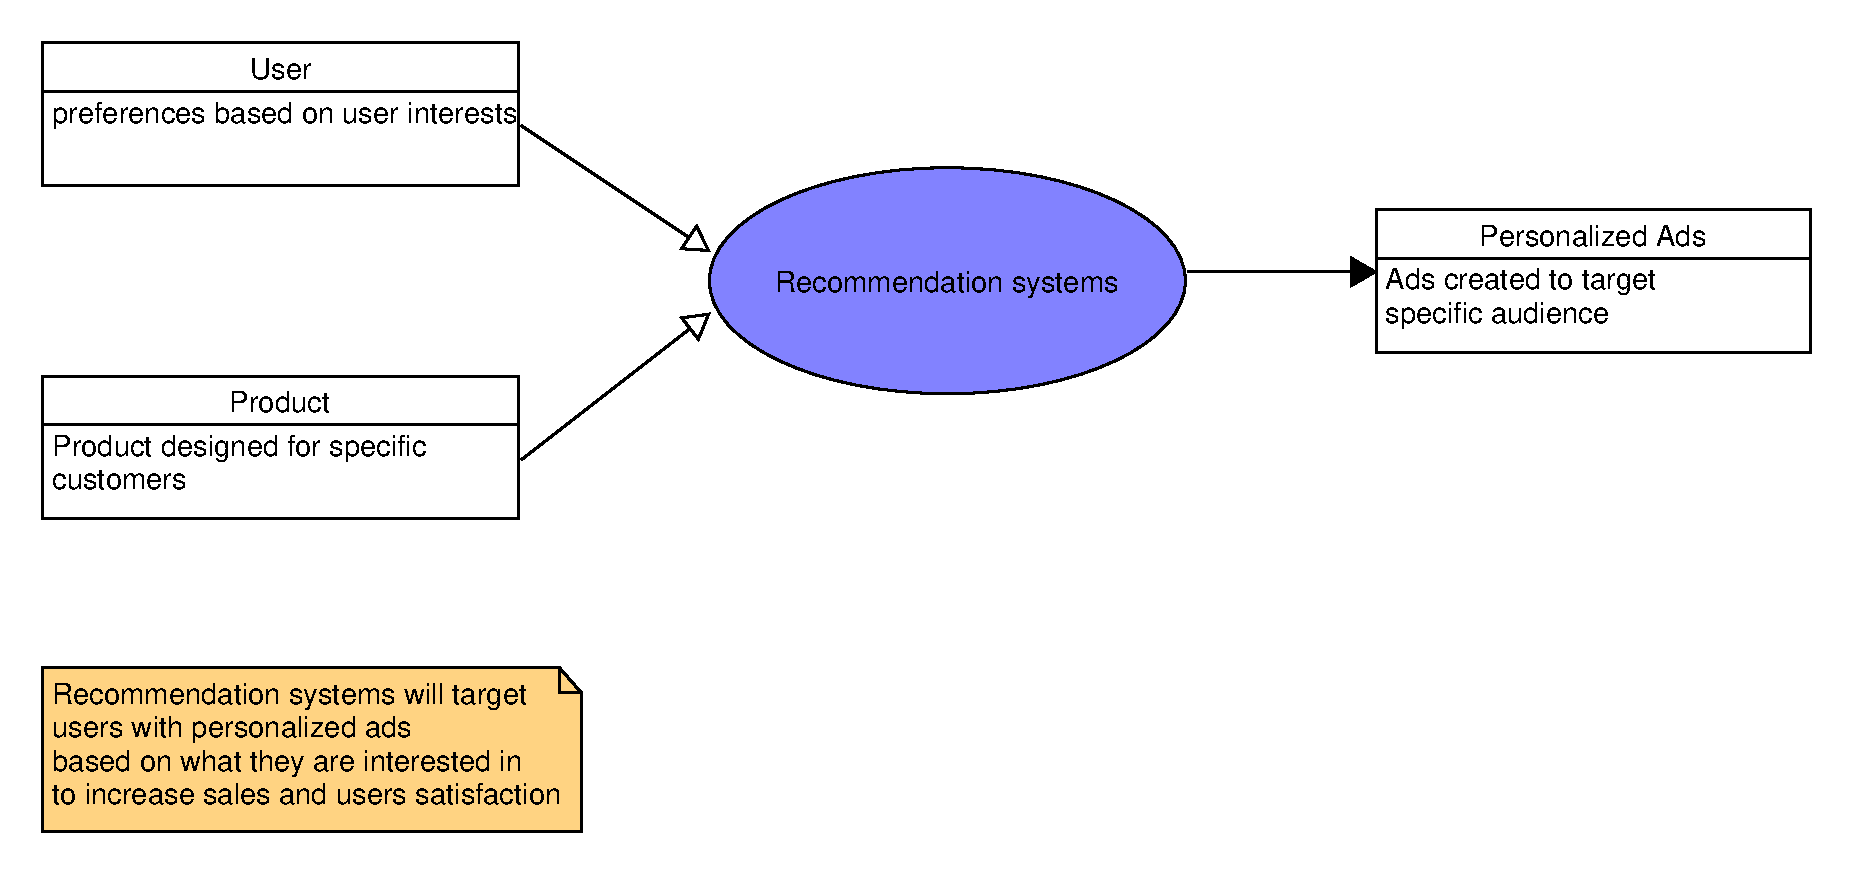
\includegraphics[width=0.75\textwidth]{diagram_2.pdf}
  %\caption{Recommendation systems role in personalized ads.}
%\ref{fig:dia2} Recommendation systems role in personalized ads.
%\end{subfigure}
%\begin{subfigure}
  %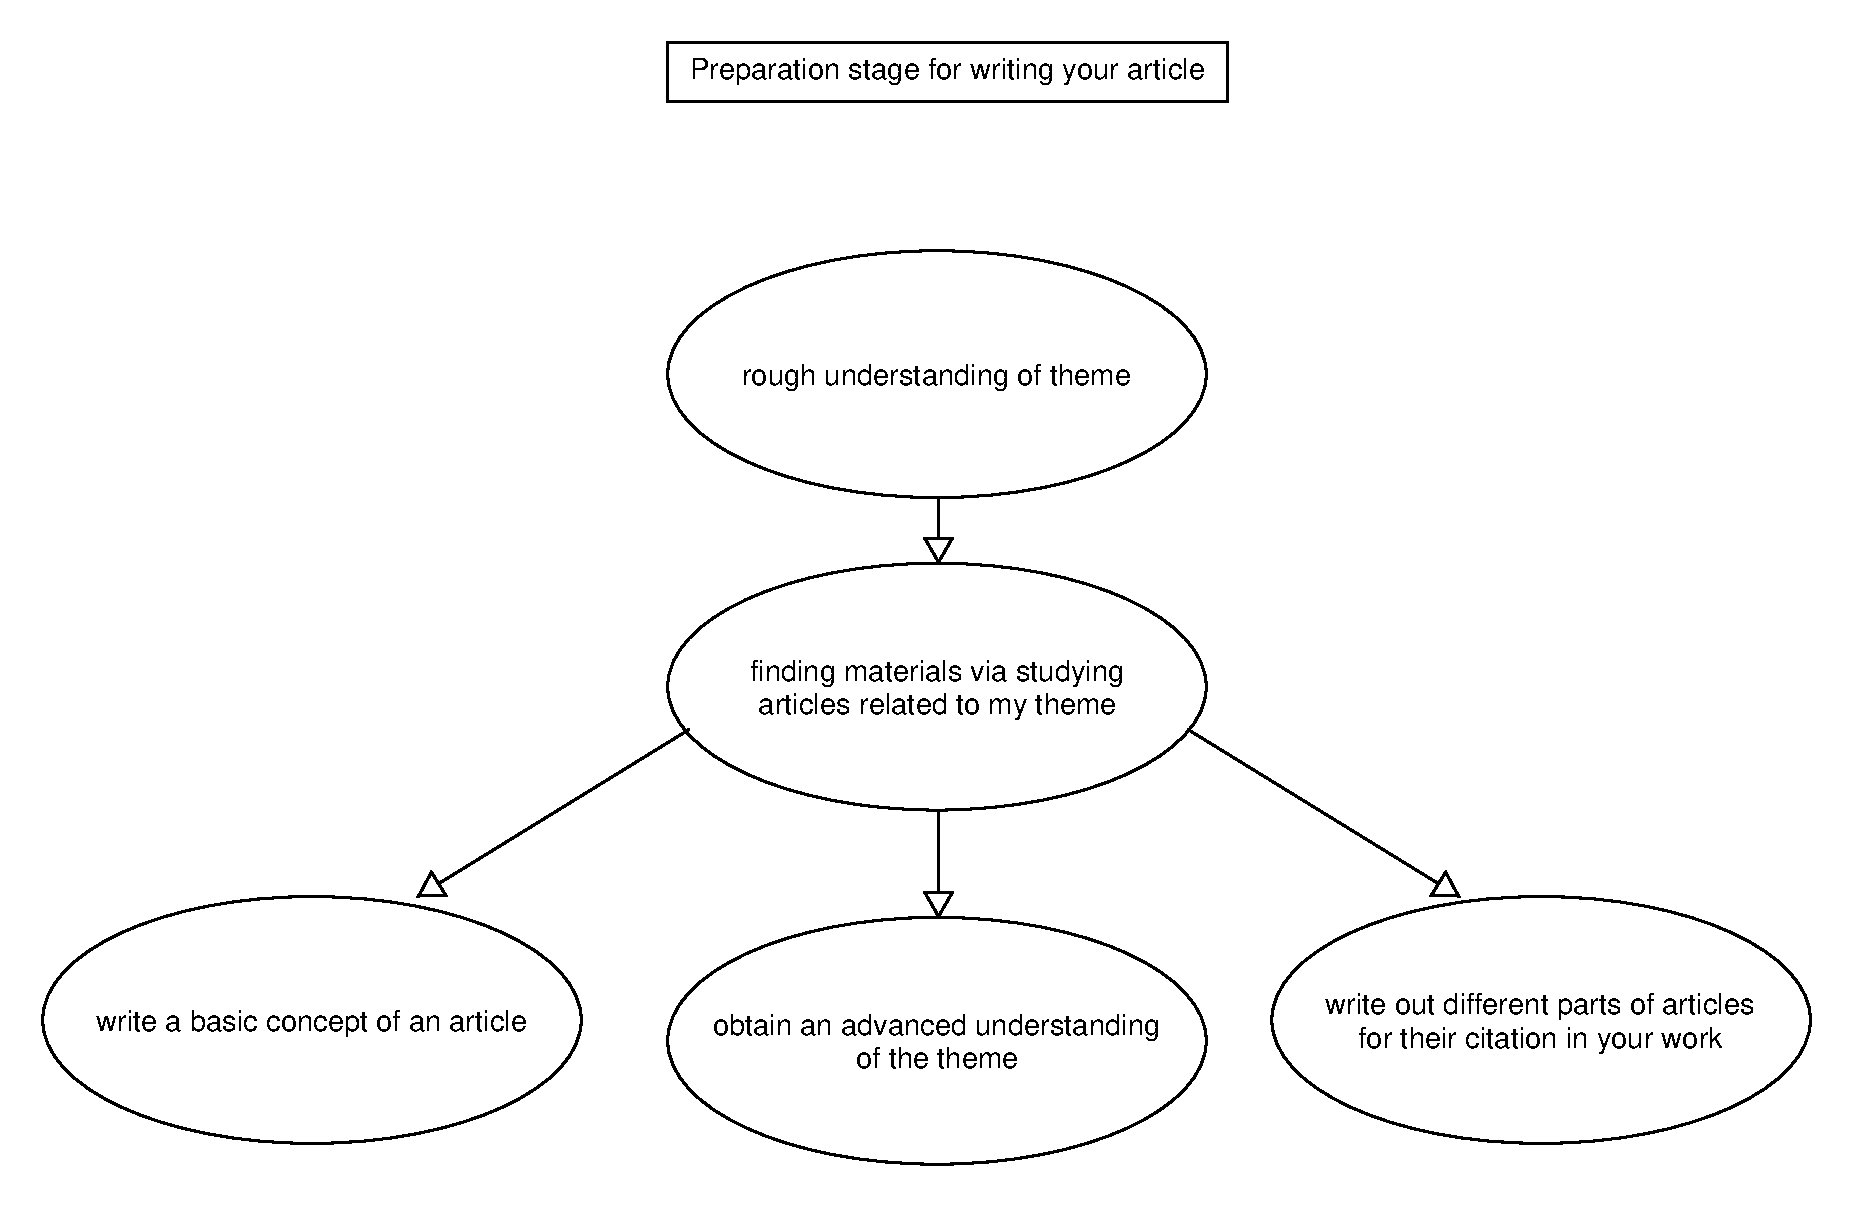
\includegraphics[width=0.75\textwidth]{diagram_1.pdf}
  %\caption{Start of work.}
  %\label{fig:dia1}
%\ref{fig:dia1} Start of work on an article.
%\end{subfigure}
%\end{figure}



\section{Second Part}

%\acknowledgement{Ak niekomu chcete poďakovať\ldots}


% týmto sa generuje zoznam literatúry z obsahu súboru literatura.bib podľa toho, na čo sa v článku odkazujete
% \bibliography{literature}
% \bibliographystyle{plain} % prípadne alpha, abbrv alebo hociktorý iný
\end{document}
